% \iffalse meta-comment
% 
% Copyright (C) 2009 by Nico Schlömer
% 
% This file may be distributed and/or modified under the
% conditions of the LaTeX Project Public License, either
% version 1.2 of this license or (at your option) any later
% version. The latest version of this license is in:
% 
%    http://www.latex-project.org/lppl.txt
% 
% and version 1.2 or later is part of all distributions of
% LaTeX version 1999/12/01 or later.
%
% \fi
%
% \iffalse
%<style>\NeedsTeXFormat{LaTeX2e}[1999/12/01]
%<style>\ProvidesPackage{auto1}
%<style>   [2009/06/15 v0.2 Auto 1 support for LaTeX]
%
%
%<*driver>
\documentclass{ltxdoc}
% \usepackage{lmodern}
\usepackage{MinionPro}
\usepackage[T1]{fontenc}
\usepackage{listings}  % include highlighted source code
\lstset{% general command to set parameter(s)
basicstyle=\ttfamily, % print whole listing small
keywordstyle=\color{uablue},
identifierstyle=,
commentstyle=\color{olive},
stringstyle=\color{uared},
showstringspaces=false,     % no special string spaces
frame=single,
language=[LaTeX]TeX
}
\usepackage{lipsum}
\usepackage{microtype}
\usepackage[british]{babel}
\usepackage{booktabs,paralist,calc}
\usepackage[unicode,bookmarks]{hyperref}
\usepackage{subfig,graphicx}
\usepackage{xcolor}
\usepackage{csquotes}
\usepackage{tikz,pgfplots}
\usepackage{tabulary}
\usepackage{eurosym}
\usepackage{siunitx}
\usepackage{listings}  % include highlighted source code
\lstset{% general command to set parameter(s)
basicstyle=\ttfamily, % print whole listing small
keywordstyle=\color{uablue},
identifierstyle=,
commentstyle=\color{olive},
stringstyle=\color{uared},
showstringspaces=false,     % no special string spaces
frame=single,
language=[LaTeX]TeX
}
\hypersetup{
  bookmarksnumbered,
  colorlinks,
  pdfborder={0 0 0},
  citecolor=vividbrown,
  urlcolor=uared75,
  pdftitle={LaTeX beamer theme for the Universiteit Antwerpen},
  pdfauthor={Nico Schl\"omer},
  pdfkeywords={LaTeX, Beamer, Universiteit Antwerpen}
}


\usepackage[%
bibtex8=true,
hyperref=auto
]{biblatex}
\bibliography{bibtex/beamerstyleUa}


% =========================================================================
% define colors
% =========================================================================
% see \acro{PMS}-\acro{CMYK}-\acro{RGB} conversion chart at http://www.zedimage.com/pms-cmyk-hex.php
\definecolor{uablue}{cmyk}{1,0.25,0,0.5}
\colorlet{uablue100}{uablue}
\colorlet{uablue75} {uablue!75!white}
\colorlet{uablue50} {uablue!50!white}
\colorlet{uablue25} {uablue!25!white}
\colorlet{uablue10} {uablue!10!white}
\colorlet{uablue5}  {uablue!5!white}

\definecolor{uared}{cmyk}{0,1,0.6,0.37}
\colorlet{uared100}{uared}
\colorlet{uared75} {uared!75!white}
\colorlet{uared50} {uared!50!white}
\colorlet{uared25} {uared!25!white}
\colorlet{uared10} {uared!10!white}
\colorlet{uared5}  {uared!5!white}

\definecolor{vividbrown}{RGB}{215,154,70}
\colorlet{vividbrown100}{vividbrown}
\colorlet{vividbrown75} {vividbrown!75!white}
\colorlet{vividbrown50} {vividbrown!50!white}
\colorlet{vividbrown25} {vividbrown!25!white}
\colorlet{vividbrown10} {vividbrown!10!white}
\colorlet{vividbrown5}  {vividbrown!5!white}
% =========================================================================


\newcommand\colorsquare[2]{\colorbox{#2}{\rule{0mm}{#1}\rule{#1}{0mm}}}
\newcommand\colorsquareseries[2]{%
\colorsquare{#1}{#2}%
\colorsquare{#1}{#2!75|white}%
\colorsquare{#1}{#2!50|white}%
\colorsquare{#1}{#2!15!white}%
\colorsquare{#1}{#2!10!white}%
\colorsquare{#1}{#2!5!white}%
}

% % =========================================================================
% % A colorwheel as generated by http://www.colorschemer.com/online.html
% % with the input value \acro{RGB}(0,112,128).
% % Neither of the two \acro{UA} colors will exactly fit in there, but both approximately
% % at positions (1,1) and (3,4), respectively.
% % Pick the complimentary colors from that wheel.
% \definecolor{col11}{RGB}{  0,111,128}  % approx. uablue
% \definecolor{col12}{RGB}{  0, 47,128}
% \definecolor{col13}{RGB}{ 17,  0,128}
% \definecolor{col14}{RGB}{ 81,  0,128}
% 
% \definecolor{col21}{RGB}{  0,128, 81}
% \definecolor{col22}{RGB}{  0,164,189}
% \definecolor{col23}{RGB}{  0,217,250}
% \definecolor{col24}{RGB}{128,  0,111}
% 
% \definecolor{col31}{RGB}{  0,128, 17}
% \definecolor{col32}{RGB}{250, 33,  0}
% \definecolor{col33}{RGB}{189, 25,  0}
% \definecolor{col34}{RGB}{128,  0, 47} % approx. uared
% 
% \definecolor{col41}{RGB}{ 47,128,  0}
% \definecolor{col42}{RGB}{111,128,  0}
% \definecolor{col43}{RGB}{128, 81,  0}
% \definecolor{col44}{RGB}{128, 17,  0}
% % =========================================================================

\usepackage[amsthm]{ntheorem}
\theoremstyle{definition}
\newtheorem*{note}{Note}

\newcommand\powerpoint{Microsoft PowerPoint\textregistered}

\newcommand{\changefont}[3]{\fontfamily{#1}\fontseries{#2}\fontshape{#3}\selectfont}

\newcommand*\pkg[1]{\mbox{\textsf{#1}}}
\newcommand*\file[1]{\textsf{#1}}
\newcommand*\acro[1]{\textsc{\MakeLowercase{#1}}}
\newcommand\pdfTeX{pdf\TeX}
\pdfstringdefDisableCommands{%
  \renewcommand*\acro[1]{#1}%
}

\makeatletter
\newcommand*\option{\@ifstar\option@default\option@}
\newcommand*\option@default[1]{\option@{#1}*}
\newcommand*\option@[1]{\textsf{#1}}
\makeatother

\setlength{\leftmargini}{1em}
\setlength{\parindent}{1em}
\newcommand\tabindent{\noindent\hspace{\leftmargini}}
\newlength\optionswidth
\providecommand\newblock{}
\newenvironment{options}[1][{\makebox[\optionswidth]{}}]{%
  \settowidth{\optionswidth}{#1}%
  \global\optionswidth=\optionswidth
  \list{}{%
    \setlength{\labelwidth}{\optionswidth}%
    \setlength{\labelsep}{2\tabcolsep}%
    \setlength{\leftmargin}{\leftmargini+\labelwidth+\labelsep}%
    \setlength{\rightmargin}{0pt}%
    \setlength{\topsep}{\medskipamount}%
    \setlength{\parsep}{0pt}%
    \setlength{\itemsep}{0pt}%
    \renewcommand*\makelabel[1]{%
      \parbox[t]{\labelwidth}{\raggedright\hspace{0pt}##1}}%
    \renewcommand\newblock{\medskip}%
    \raggedright
  }%
}{%
  \endlist
}

\newlength\figurewidth
\newlength\figureheight

\setcounter{secnumdepth}{2}
\setcounter{tocdepth}{2}

\EnableCrossrefs
\CodelineIndex
\RecordChanges
% \AtBeginDocument{\OnlyDescription}
\begin{document}
  \DocInput{ua-beamer.dtx}
\end{document}
%</driver>
% \fi
%
% \changes{v0.2}{2009/06/15}{Proper LaTeX documentation}
% \changes{v0.1}{2009/00/00}{Initial version}
%
% \GetFileInfo{ua-beamer.sty}
%
% \DoNotIndex{\#,\$,\%,\&,\@,\\,\{,\},\^,\_,\~,\ }
% \DoNotIndex{\@ne}
% \DoNotIndex{\advance,\begingroup,\catcode,\closein}
% \DoNotIndex{\closeout,\day,\def,\edef,\else,\empty,\endgroup}
%
% \title{A \pkg{beamer} presentation class theme for the Universiteit Antwerpen}
% \author{Nico~Schl\"omer}
% \date{\fileversion\ -- \filedate}
%
% \maketitle
%
% \begin{abstract}
% This is a theme for the \LaTeX{} \pkg{beamer} class for presentations. It has been designed to  match the official \acro{UA} templates for \powerpoint{} while doing away with some of the shortcomings of it within the \pkg{beamer} framework. If you would like to give a scientific presentation with all the benefits you get from using \LaTeX{}, this theme is for you.\footnote{Note that there exists another \pkg{beamer} theme for the Universiteit Antwerpen designed by \textsc{Kris Ven} \cite{Ven::BTU}, which has many more options than this package. In contrast to this theme, it is not designed with compliance to the official themes in mind.}
% 
% % Moreover, as of this writing, it is not known to the author whether or not that theme is still being made available for download.
% \end{abstract}
% \tableofcontents
%
% \section{Installation}
% 
% \subsection{Requirements}
% The theme is an addendum for the \LaTeX{} \pkg{beamer} class, hence it is assumed that you have a running \LaTeX{} installation together with
% the \pkg{beamer} package \cite{Tantau:2008:LBC} and its dependencies. If not already the case, it will also certainly be a good idea to make
% yourself familiar with the \pkg{beamer} class. The excellent manual \cite{Tantau:2007:UGB} is will serve you well.
% %Basically, it is straightforward to adapt your \pkg{beamer} presentation to the official \acro{UA} design. After placing files somewhere into the
% \TeX{} file tree (see above), the only this necessary 
% 
% \subsection{Getting the package}
% 
% The package is distributed on the maintainer's website \cite{Schloemer:2009:website}. You can get the latest releases there, as well as
% additional information about the package. If you would like to stay on the bleeding edge of development, you can have read access to the
% Subversion repository by typing
% \begin{quote}
% |$ svn co svn://macos.cmi.ua.ac.be:/home/wins/toegw/nschloe/svnrepos/ua-beamer|
% \end{quote}
% 
% 
% \subsection{First run}
% Once you have the files, all that is required for the theme to work is putting the files into a directory where \LaTeX{} can find them. If you
% would like to install it for one user only, this would typically be |~/texmf/| (on Unix). For all other options please refer to the
% documentation of your \LaTeX{} package manager.
% 
% You can check if \LaTeX{} finds the files in its directories by, for example, looking for the file |beamerfontthemeUniversiteitAntwerpen.sty|,
% \begin{quote}
% |$ kpsewhich beamerfontthemeUniversiteitAntwerpen.sty|
% \end{quote}
% If everything seems okay, you can check whether you can actually produce a presentation with the \acro{UA} theme by either creating a minimal test
% file (see listing \ref{listing:minex}) or by compiling the \LaTeX-document provided in the |example/| folder of this package. 
% 
% 
% \begin{figure}
% \centering
% \setlength{\figurewidth}{5cm}
% \subfloat[][The first two pages with light theming (default).]{%
% \frame{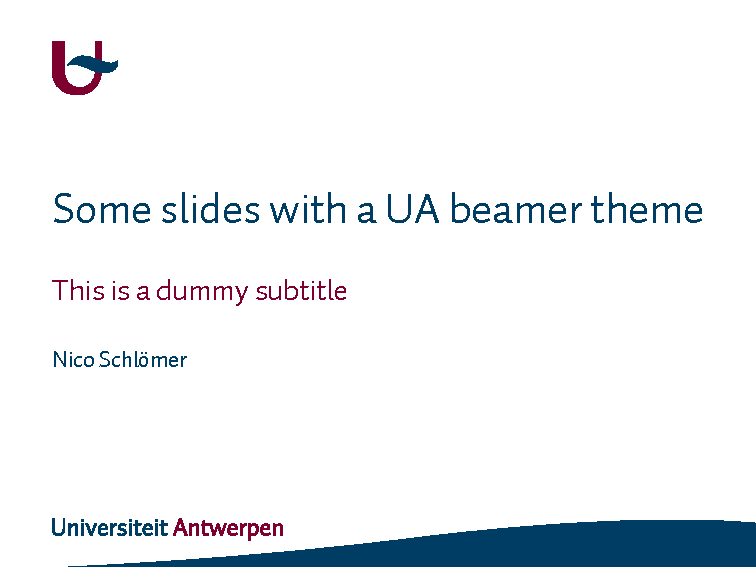
\includegraphics[width=\figurewidth]{figures/light-page1}}%
% \qquad
% \frame{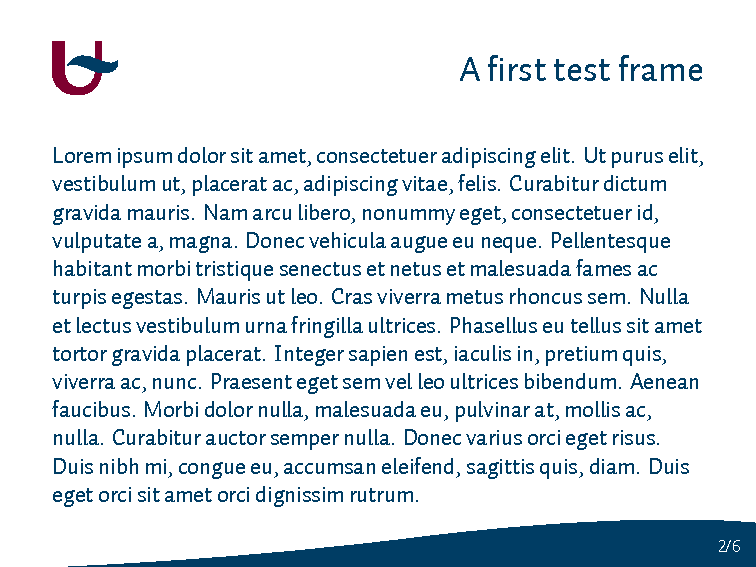
\includegraphics[width=\figurewidth]{figures/light-page2}}%
% }
% 
% \subfloat[][The first two pages with dark theming (option option{dark}).]{%
% \frame{
\includegraphics[width=\figurewidth]{figures/dark-page1}}%
% \qquad
% \frame{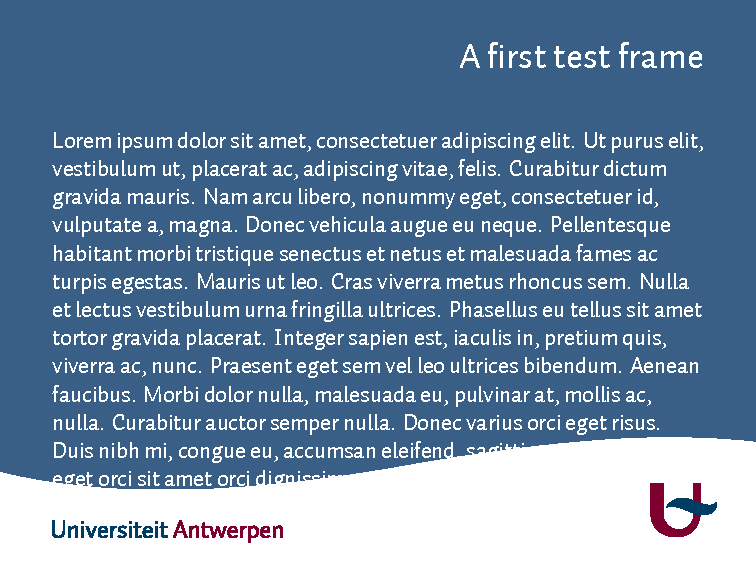
\includegraphics[width=\figurewidth]{figures/dark-page2}}%
% }
% 
% \caption{The first two pages of \acro{PDF} output of the example file in example/, with light and dark theming. The theme is loaded with the
% option \textsf{framenumber} and the \pkg{beamer} package itself with option{compress}. Note that it is also possible the combine the dark title page
% with light content pages (option option{darktitle}, see below).}
% \label{fig:example1}
% \end{figure}
% 
% \begin{note}
% You might need to install more \LaTeX{} packages when running the provided example file (e.g., the \pkg{lipsum} package).
% \end{note}
% 
% \begin{lstlisting}[float,caption={A minimalistic test file for the \acro{UA} Beamer theme.},captionpos=b,label=listing:minex,abovecaptionskip=\bigskipamount]
\documentclass{beamer}

\usetheme{UniversiteitAntwerpen}

\begin{document}

\begin{frame}
Hello world!
\end{frame}

\end{document}
% \end{lstlisting}
%
% \section{Options}
%
% The theme comes with several options, all of which can be given in a comma-separated list like in
% \begin{quote}
% |\usetheme[|\textit{<options>}|]{UniversiteitAntwerpen}|
% \end{quote}
%
% Just like the Universiteit Antwerpen itself provides two different flavors of \powerpoint{} presentations, one
% with a light background and one with a darker, this \pkg{beamer} themes inherits options for both. By default, the theme applies the light
% theme, this options switches to the dark counterpart. See figure \ref{fig:example1}.
% The default settings are marked with an asterisk*.
% 
% \begin{options}[\option{proportional}, \option{prop}]
% \item[\option*{light}]      use light version
% \item[\option{dark}]        use dark (blue) version
% \end{options}
% \begin{options}[\option{proportional}, \option{prop}]
% \item[\option{darktitle}]   use title page of the dark theme
% \end{options}
% \begin{options}[\option{proportional}, \option{prop}]
% \item[\option{framenumber}]    With the light scheme, the \option{framenumber} option makes sure that the number of the current frame as well as the total number of frames is displayed in the right lower corner of each frame. Does not do anything with the dark variant (see option \option{dark})
% \end{options}
% 
% \begin{note}
% The \pkg{beamer} option \option{compress} is respected in the sense that, if it is provided, header and footer will take less space such that
% there is more space for actual frame content.
% \end{note}
%
% \section{Colors}\label{sec:colors}
% 
% \subsection{Background on the official colors}
% 
% \begin{note}
% If you don't care about the technical details, you can skip this and directly go to subsection \ref{subsection:usingthecolors}.
% \end{note}
% 
% The two official colors of the \acro{UA}, a blue and a red tone, are originally given in \acro{PMS} format, a \emph{proprietary} format issued
% by the Pantone Inc.\ corporation. One particular feature of the \acro{PMS} color format is that it is, as opposed to \acro{RGB} or \acro{CMYK},
% \emph{device independent}. This means that the definition of the color does not consist of instructions such as \enquote{put 37\% red, 12\%
% green, and 45\% blue and mix it all together}, but really is a concise description of what the final result, be it printed or displayed,
% physically looks like on the medium under determined ambient light conditions.
% 
% The \acro{PMS} format is richer than \acro{RGB} in the sense that it can embrace fluorescence effects, gold or silver shine, special coatings
% (matte and brilliant), in general everything that has to do with the actual appearance of the color on the medium. It comes thus as no surprise
% that there is no (exact) mapping between the \acro{PMS} and \acro{RGB} color spaces; more specifically: the mapping -- if it exists -- is
% device-dependent.
% 
% The \emph{only} way to get a perfect \acro{PMS} 1955 red, for example, is to have a the plot file ready with the (proprietary) \acro{PMS} color
% information in it, and have it printed on a \acro{PMS}-ready printer which needs to be filled the special \acro{PMS} 1955 ink beforehand. This
% process is eponymous for colors which are not composed of different types of (yellow, blue, red) inks: they are called \emph{single-spot
% colors}, and most Pantone\textsuperscript{\textregistered} colors are of such kind.
% 
% 
% \subsection{Conversion to \acro{RGB}/\acro{CMYK}}
% 
% When the computer screen or any other non-\acro{PMS}-ready medium is the primary output source, having such rigorous rules may be rather
% obstructive. To overcome such restrictions, many vendors of graphical software try to translate \acro{PMS} into \acro{RGB}/\acro{CMYK} by
% making use of special monitor color calibration data (e.g., \acro{ICC} color profiles). Unfortunately, if files containing
% \acro{PMS} color information are displayed (printed) with programs (printers) which do not support \acro{PMS} mechanisms (which is most often
% the case in non-professional environments), the color output will look disturbed. On top of that, and surprisingly for the novice, the output
% will look disturbed in different ways on different screens (printers) because of the inherent device-dependence of \acro{PMS}.
% 
% %To overcome the undesired side-effects of working with the official \acro{UA} corporate design in a non-\acro{PMS} environment (like most beamers and
% computer screens should provide),
% That is why this theme aims to use non-\acro{PMS} versions of the \acro{UA}'s official colors, including modified versions of the logos.
% 
% \begin{table}
% \centering
% \newlength{\boxsize}
% \setlength{\boxsize}{2cm}
% 
% \begin{tabular}{cccc}
% \definecolor{uablue11}{RGB}{  0, 61,100}
% \colorbox{uablue11}{\rule{0mm}{\boxsize}\rule{\boxsize}{0mm}}
% &
% \definecolor{uablue12}{cmyk}{1,0.3,0,0.62}
% \colorbox{uablue12}{\rule{0mm}{\boxsize}\rule{\boxsize}{0mm}}
% &
% \definecolor{uablue13}{RGB}{0,96,128}
% \colorbox{uablue13}{\rule{0mm}{\boxsize}\rule{\boxsize}{0mm}}
% &
% \definecolor{uablue14}{cmyk}{1,0.25,0,0.5}
% \colorbox{uablue14}{\rule{0mm}{\boxsize}\rule{\boxsize}{0mm}}\\[2mm]
% \definecolor{uared11}{RGB}{126,  0, 47}
% \colorbox{uared11}{\rule{0mm}{\boxsize}\rule{\boxsize}{0mm}}
% &
% \definecolor{uared11}{cmyk}{0,1,0.54,0.46}
% \colorbox{uared11}{\rule{0mm}{\boxsize}\rule{\boxsize}{0mm}}
% &
% \definecolor{uared11}{RGB}{161,0,64}
% \colorbox{uared11}{\rule{0mm}{\boxsize}\rule{\boxsize}{0mm}}
% &
% \definecolor{uared11}{cmyk}{0,1,0.6,0.37}
% \colorbox{uared11}{\rule{0mm}{\boxsize}\rule{\boxsize}{0mm}}
% \end{tabular}
% 
% \caption{\acro{PMS} 302 and \acro{PMS} 1955 translated to \acro{CMYK}/\acro{RGB} in different ways. Left to right: \acro{UA} website \cite{KAN::}
% \acro{RGB}, \acro{UA} website \cite{KAN::} \acro{CMYK}, conversion chart \cite{::TDC} \acro{RGB}, conversion chart \cite{::TDC} \acro{CMYK}. To
% determine which version is closest to the actual colors \acro{PMS} 1955 and \acro{PMS} 302 on your monitor/printer/beamer, you would need a
% physical color sample (such as provided on the Pantone\textsuperscript{\textregistered} charts) to compare.}
% \label{table:reds-blues}
% \end{table}
% 
% Now, as explained above there is no device-independent conversion between the original \acro{PMS} directives and the \acro{CMYK} color space;
% several tables exist which are valid for different work environments. On the official sites of the \acro{UA} \cite{KAN::}, you'll find particular
% \acro{RGB} and \acro{CMYK} values, other resources, e.g., \cite{::TDC}, provide other numbers (see table \ref{table:reds-blues}).
% 
% For the sake of consistency between \acro{RGB} and \acro{CMYK} values, the \pkg{beamer} theme uses the \acro{CMYK} values for \acro{PMS} 302
% and \acro{PMS} 1955 provided on \cite{::TDC} for reference (see table \ref{table:reds-blues}, last column, and table \ref{table:allcolors}).
% 
% \subsection{Using the colors}\label{subsection:usingthecolors}
% 
% 
% Getting a consistent look-and-feel throughout your presentations requires sticking to a particular style scheme, most of which is being
% implemented in the \pkg{beamer} style file already. One particular aspect, though, can only be controlled by the user, and that is the colors
% that are used in the running text, tables, and figures.
% 
% Although essentially consistent of only two colors, within \pkg{beamer} referred to as |uablue! and |uared!, provide more
% diversity than one might expect and should be  \emph{exclusively} used  in all the slides. The user should be aware that this directive
% includes \emph{tables, figures, and graphics of most kinds}. For an example of usage see figure \ref{fig:coloredgraphs}.
% 
% \begin{figure}
% \setlength{\figurewidth}{10cm}
% \setlength{\figureheight}{5cm}
% \centering
% \begin{tikzpicture}

% Axis at [0.13 0.11 0.78 0.81]
\begin{axis}[
axis on top,
scale only axis,
width=\figurewidth,
height=\figureheight,
xmin=0, xmax=10,
ymin=0, ymax=7
]

\addplot [
color=uablue,
solid,
line width=1pt
] coordinates{
 (0,5.23398) (1,4.38268) (2,4.69238) (3,4.32081) (4,3.54144) (5,3.72536) (6,3.16156) (7,2.59604) (8,2.20231) (9,2.60195) (10,1.60575)
};

\addplot [
color=uared,
solid,
line width=1pt
] coordinates{
 (0,2.02709) (1,2.02644) (2,1.68711) (3,1.84761) (4,1.78782) (5,1.24044) (6,1.26026) (7,0.992143) (8,0.859557) (9,0.689706) (10,0.36891)
};

\addplot [
color=uablue50,
solid,
line width=1pt
] coordinates{
 (0,3.2703) (1,3.30947) (2,3.74723) (3,3.45218) (4,3.3806) (5,3.13813) (6,2.81847) (7,2.79316) (8,2.64385) (9,3.01041) (10,2.72024)
};

\addplot [
color=uared50,
solid,
line width=1pt
] coordinates{
 (0,5.49163) (1,4.97712) (2,5.031) (3,5.42669) (4,5.41402) (5,5.4996) (6,5.311) (7,5.34227) (8,5.46331) (9,5.46677) (10,5.12875)
};

\addplot [
color=uablue25,
solid,
line width=1pt
] coordinates{
 (0,5.56199) (1,5.2627) (2,5.27883) (3,5.38474) (4,5.90686) (5,6.11345) (6,6.04402) (7,6.36515) (8,6.62563) (9,6.38024) (10,6.33876)
};

\addplot [
color=uared25,
solid,
line width=1pt
] coordinates{
 (0,3.7947) (1,4.08811) (2,4.28361) (3,4.45264) (4,4.46625) (5,5.28088) (6,5.32715) (7,5.54452) (8,5.439) (9,5.99242) (10,6.35941)
};

\addplot [
color=vividbrown,
solid,
line width=1pt
] coordinates{
 (0,1.43939) (1,1.51392) (2,2.30537) (3,2.05355) (4,3.05479) (5,2.9632) (6,3.16279) (7,3.3234) (8,4.15725) (9,4.278) (10,4.78022)
};

\end{axis}

\end{tikzpicture}

% \caption{Example usage of the official colors within a set of graphs, using also the exception color.}
% \label{fig:coloredgraphs}
% \end{figure}
% 
% If you need to emphasize a particular aspect in your slides (graphs, tables), you can (within \pkg{beamer}) use the |\alert{}| macro (e.g.,
% |\alert{This is alerted text.}|). For the situation where something needs to stick out in a pie chart, for example, where the ordinary colors
% (\acro{UA} blue and red) have been used up already, a third color has been added (see table \ref{table:allcolors}). It is to be used scarcely
% and strictly for highlighting purposes (see, for example, figure \ref{fig:coloredgraphs}).
% 
% 
% \begin{table}
% \setlength{\figurewidth}{12mm}
% \centering
% \begin{tabulary}{\textwidth}{LCCC}\toprule
% Color sample & \colorsquare{\figurewidth}{uablue100} & \colorsquare{\figurewidth}{uablue75} & \colorsquare{\figurewidth}{uablue50}\\
% \acro{CMYK} & (100, 30, 0, 62) & (75, 23, 0, 47) & (50, 15, 0, 31)\\
% \acro{RGB}  & (0, 61, 100)     & (40, 128, 158)  & (96, 166, 191)\\
% \pkg{beamer} name & |uablue100| & |uablue75| & |uablue50|\\[3mm]
% Color sample & \colorsquare{\figurewidth}{uablue25} & \colorsquare{\figurewidth}{uablue10} & \colorsquare{\figurewidth}{uablue5}\\
% \acro{CMYK} & (25, 8, 0, 16)  & (10, 3, 0, 6)   & (5, 2, 0, 3)\\
% \acro{RGB}  & (166, 209, 222) & (218, 235, 242) & (235, 245, 247)\\
% \pkg{beamer} name & |uablue25| & |uablue10| & |uablue5|\\\midrule
% 
% Color sample & \colorsquare{\figurewidth}{uared100} & \colorsquare{\figurewidth}{uared75} & \colorsquare{\figurewidth}{uared50}\\
% \acro{CMYK} & (0, 100, 54, 46) & (0, 75, 41, 35) & (0, 50, 27, 23)\\
% \acro{RGB}  & (161, 0, 64)     & (184, 46, 101)  & (207, 103, 145)\\
% \pkg{beamer} name & |uared100| & |uared75| & |uared50|\\[3mm]
% Color sample & \colorsquare{\figurewidth}{uared25} & \colorsquare{\figurewidth}{uared10} & \colorsquare{\figurewidth}{uared5}\\
% \acro{CMYK} & (0, 25, 14, 12)  & (0, 10, 5, 5)   & (0, 5, 3, 2)\\
% \acro{RGB}  & (232, 174, 197) & (245, 220, 230) & (250, 237, 242)\\
% \pkg{beamer} name & |uared25| & |uared10| & |uared5|\\\midrule
% 
% Color sample & \colorsquare{\figurewidth}{vividbrown} & \colorsquare{\figurewidth}{vividbrown75} & \colorsquare{\figurewidth}{vividbrown50}\\
% \acro{CMYK} & (0, 28, 67, 16) & (0, 20, 48, 12) & (0, 13, 31, 8)\\
% \acro{RGB}  & (215, 154, 70) & (225, 179, 116)  & (235, 205, 163)\\
% \pkg{beamer} name & |vividbrown100| & |vividbrown75| & |vividbrown50|\\[3mm]
% Color sample & \colorsquare{\figurewidth}{vividbrown25} & \colorsquare{\figurewidth}{vividbrown10} & \colorsquare{\figurewidth}{vividbrown5}\\
% \acro{CMYK} & (0, 6, 15, 4) & (0, 2, 6, 2) & (0, 1, 3, 1)\\
% \acro{RGB}  & (245, 230, 209)  & (251, 245, 237) & (253, 250, 246)\\
% \pkg{beamer} name & |vividbrown25| & |vividbrown10| & |vividbrown5|\\\bottomrule
% \end{tabulary}
% 
% \caption{Overview over the two main colors used in theme as well as the third color for exceptions and highlighting.}
% \label{table:allcolors}
% \end{table}
%
%
% \section{Fonts}
% 
% To stick entirely to the corporate design of the Universiteit Antwerpen, one is bound to use the official font series \enquote{Auto} of Underware \cite{Underware::ATI}. As stated on the \acro{UA} website, \textquote[KAN::T][.]{Een weloverwogen en consequente gebruik van typografie is de ruggengraat van een huisstijl.} (A deliberate and consistent use of typography is the backbone of a corporate design.). 
% 
% Unfortunately, these fonts are not freely available, not even for university members. In order to make use of the most basic fonts, it would be enough to dispose of the \enquote{Auto 1 office package}, available for \EUR{200} per personal license. The files can be purchased either in TrueType OpenType format (|.ttf|) or PostScript Type 1 format (|.pfm|). While the PostScript format is native to \LaTeX{}, it TrueType fonts can also be used natively in \LaTeX{} with pdf\LaTeX; installation instructions are plenty (e.g., \cite{Rakityansky::TTF}).
% 
% 
% 
% \begin{table}
% \centering
% \newcommand\quickfox{The quick brown fox jumps over the lazy dog.}
% \newcommand\ligatures{ff fl fi To AV \'e \`a \"a \"o \"u \"{i} \oe{} \ae{} \ss{} - -- --- ?`? \% \& @}
% \begin{tabular}{lll}\toprule
% weight  & shape  & sample\\\midrule
% light   & normal            & {\changefont{fa1-OsF}{l}{n}\quickfox}\\
%         &                   & {\changefont{fa1-OsF}{l}{n}\ligatures}\\
%         & italic            & {\changefont{fa1-OsF}{l}{it}\quickfox}\\
%         &                   & {\changefont{fa1-OsF}{l}{it}\ligatures}\\
%         & small caps        & {\changefont{fa1-OsF}{l}{sc}\quickfox}\\
%         &                   & {\changefont{fa1-OsF}{l}{sc}\ligatures}\\
%         & italic small caps & {\changefont{fa1-OsF}{l}{itsc}\quickfox}\\
%         &                   & {\changefont{fa1-OsF}{l}{itsc}\ligatures}\\\midrule
% regular & normal            & {\changefont{fa1-OsF}{m}{n}\quickfox}\\
%         &                   & {\changefont{fa1-OsF}{m}{n}\ligatures}\\
%         & italic            & {\changefont{fa1-OsF}{m}{it}\quickfox}\\
%         &                   & {\changefont{fa1-OsF}{m}{it}\ligatures}\\
%         & small caps        & {\changefont{fa1-OsF}{m}{sc}\quickfox}\\
%         &                   & {\changefont{fa1-OsF}{m}{sc}\ligatures}\\
%         & italic small caps & {\changefont{fa1-OsF}{m}{itsc}\quickfox}\\
%         &                   & {\changefont{fa1-OsF}{m}{itsc}\ligatures}\\\midrule
% bold    & normal            & {\changefont{fa1-OsF}{b}{n}\quickfox}\\
%         &                   & {\changefont{fa1-OsF}{b}{n}\ligatures}\\
%         & italic            & {\changefont{fa1-OsF}{b}{it}\quickfox}\\
%         &                   & {\changefont{fa1-OsF}{b}{it}\ligatures}\\
%         & small caps        & {\changefont{fa1-OsF}{b}{sc}\quickfox}\\
%         &                   & {\changefont{fa1-OsF}{b}{sc}\ligatures}\\
%         & italic small caps & {\changefont{fa1-OsF}{b}{itsc}\quickfox}\\
%         &                   & {\changefont{fa1-OsF}{b}{itsc}\ligatures}\\\midrule
% black   & normal            & {\changefont{fa1-OsF}{c}{n}\quickfox}\\
%         &                   & {\changefont{fa1-OsF}{c}{n}\ligatures}\\
%         & italic            & {\changefont{fa1-OsF}{c}{it}\quickfox}\\
%         &                   & {\changefont{fa1-OsF}{c}{it}\ligatures}\\
%         & italic            & {\changefont{fa1-OsF}{c}{itlf}\quickfox}\\
%         &                   & {\changefont{fa1-OsF}{c}{itlf}\ligatures}\\
%         & small caps        & {\changefont{fa1-OsF}{c}{sc}\quickfox}\\
%         &                   & {\changefont{fa1-OsF}{c}{sc}\ligatures}\\
%         & italic small caps & {\changefont{fa1-OsF}{c}{itsc}\quickfox}\\
%         &                   & {\changefont{fa1-OsF}{c}{itsc}\ligatures}\\\bottomrule
% \end{tabular}
% 
% \caption{Samples of the font Auto 1 of Underware. All regular and italic versions are available with lining and text figures.}
% \end{table}
%
% \section{Version history}
%
% Version 0.2: ...\\
% Version 0.1: Initial release\\
%
% \printbibliography
%
% \StopEventually{\PrintIndex}
%
%
% \newpage
% \section{Implementation}
%
% \subsection{Main style file}
%
% \subsubsection{Options}
%
%    \begin{macrocode}
%<*style>
\DeclareOptionBeamer{compress}{\beamer@compresstrue}

\newif\ifbeamer@dark
\beamer@darkfalse
\DeclareOptionBeamer{dark}{\beamer@darktrue}

\newif\ifbeamer@darktitle
\beamer@darktitlefalse
\DeclareOptionBeamer{darktitle}{\beamer@darktitletrue}

\newif\ifbeamer@framenumber
\beamer@framenumberfalse
\DeclareOptionBeamer{framenumber}{\beamer@framenumbertrue}

\ProcessOptionsBeamer
%    \end{macrocode}
%
% Include the other style files.
%
%    \begin{macrocode}
\mode<presentation>

\useinnertheme{UniversiteitAntwerpen}
\usefonttheme {UniversiteitAntwerpen}
\usecolortheme{UniversiteitAntwerpen}
\useoutertheme{UniversiteitAntwerpen}

\mode
<all>
%</style>
%    \end{macrocode}
%
%
% \subsection{Color style file}
%
%    \begin{macrocode}
%<*color>
\mode<presentation>
%    \end{macrocode}
%
% Define standard colors based on the values given on \cite{KAN::}; compare section~\ref{sec:colors}.
%
%    \begin{macrocode}
\definecolor{uablue}{RGB}{0,61,100}
\colorlet{uablue100}{uablue}
\colorlet{uablue75} {uablue!75!white}
\colorlet{uablue50} {uablue!50!white}
\colorlet{uablue25} {uablue!25!white}
\colorlet{uablue10} {uablue!10!white}
\colorlet{uablue5}  {uablue!5!white}

\definecolor{uared}{RGB}{126,0,47}
\colorlet{uared100}{uared}
\colorlet{uared75} {uared!75!white}
\colorlet{uared50} {uared!50!white}
\colorlet{uared25} {uared!25!white}
\colorlet{uared10} {uared!10!white}
\colorlet{uared5}  {uared!5!white}

\definecolor{vividbrown}{RGB}{215,154,70}
\colorlet{vividbrown100}{vividbrown}
\colorlet{vividbrown75} {vividbrown!75!white}
\colorlet{vividbrown50} {vividbrown!50!white}
\colorlet{vividbrown25} {vividbrown!25!white}
\colorlet{vividbrown10} {vividbrown!10!white}
\colorlet{vividbrown5}  {vividbrown!5!white}
%    \end{macrocode}
%
% Define the \pkg{beamer} colors, dependent on whether or not the \option{dark} option was given.
%
%    \begin{macrocode}
\ifbeamer@dark%

  \setbeamercolor{structure}{fg=white}%
  \setbeamercolor{normal text}{fg=white}%
  \setbeamercolor{frametitle}{fg=white}%

\else%

  \setbeamercolor{structure}{fg=uablue}%
  \setbeamercolor{normal text}{fg=uablue}%
  \setbeamercolor{frametitle}{fg=uablue}%

  \setbeamercolor{frame number in foot}{fg=white}%

  \ifbeamer@darktitle%
      \setbeamercolor{title}{fg=white}%
      \setbeamercolor{subtitle}{fg=white}%
  \else
      \setbeamercolor{subtitle}{fg=uared}%
  \fi

\fi
%    \end{macrocode}
%
% Define the \pkg{alert} color.
%
%    \begin{macrocode}
\setbeamercolor{alerted text}{fg=uared}
%    \end{macrocode}
%
% Define the block colors.
%
%    \begin{macrocode}
\setbeamercolor{block title}{use=structure,fg=white,bg=uablue}
\setbeamercolor{block title alerted}{use=alerted text,fg=white,bg=uared}
\setbeamercolor{block title example}{use=example text,fg=white,bg=uablue}

\setbeamercolor{block body}        {fg=uablue,use=block title,bg=uablue10}
\setbeamercolor{block body alerted}{fg=uablue,use=block title alerted,bg=uared10}
\setbeamercolor{block body example}{fg=uablue,use=block title example,bg=uablue10}

\mode
<all>
%</color>
%    \end{macrocode}
%
% \subsection{Font style file}
%
%    \begin{macrocode}
%<*font>
\mode<presentation>

\setbeamerfont{title}     {size=\huge}
\setbeamerfont{subtitle}  {size=\Large}
\setbeamerfont{frametitle}{size=\LARGE}

\setbeamerfont{author}{size=\normalsize}

\setbeamerfont{frame number in foot}{size=\scriptsize}

\mode
<all>
%</font>
%    \end{macrocode}
%
% \subsection{Inner theme style file}
%
%    \begin{macrocode}
%<*inner>
\mode<presentation>
%    \end{macrocode}
%
% \subsubsection*{Title page}
%
%    \begin{macrocode}
\defbeamertemplate*{title page}{ua theme}
{
  \raggedleft\usebeamerfont{title}\usebeamercolor[fg]{title}\inserttitle\par%
  \ifx\insertsubtitle\@empty%
  \else%
    \vskip2ex%
    {\raggedright\usebeamerfont{subtitle}\usebeamercolor[fg]{subtitle}\insertsubtitle\par}%
  \fi%
  \ifx\insertauthor\@empty%
  \else%
    \vskip2ex%
    {\raggedright\usebeamerfont{author}\usebeamercolor[fg]{author}\insertauthor\par}%
  \fi%
  \vfill%
}
%    \end{macrocode}
%
% \subsubsection*{Blocks}
%
%    \begin{macrocode}
\setbeamertemplate{blocks}[rounded]
%    \end{macrocode}
%
%    \begin{macrocode}
\mode
<all>
%</inner>
%    \end{macrocode}
%
% \subsection{Outer theme style file}
%
%
% This theme tries to imitate the \powerpoint{} theme as closely as possible, including of course the position of the style elements on the page.
% In \powerpoint{}, the page width is \SI{10}{}in$\times$\SI{7.5}in, while \pkg{beamer}'s assumes A4 paper (\SI{128}{\milli\meter}$\times$\SI{96}{\milli\meter}); and it is recommended not to
% mess around with that, for examply by setting
% \begin{quote}
% |\geometry{paperwidth=10.0in,paperheight=7.5in}|.
% \end{quote}
% A nasty side effect of this would be, for
% example, that fonts do not get automatically scaled and would quite tiny.
%
% Instead, define a multiplicator
% \[
% \alpha = \frac{\SI{128}{\milli\meter}}{\SI{10.0}{\in}\times 25.4\frac{\si{\milli\meter}}{in}} = \frac{64}{127}
% \]
% which scales all lengths, or rather
% \[
% \beta = \alpha\times 25.4\frac{\si{\milli\meter}}{in} = 12.8 \frac{\si{\milli\meter}}{in}
% \]
% which scales a length given in inches by $\alpha$ to a length in millimeters.
%
% Load required packages.
%    \begin{macrocode}
%<*outer>
\RequirePackage{calc}
\RequirePackage{ifthen}
%    \end{macrocode}
%
%    \begin{macrocode}
\mode<presentation>
%    \end{macrocode}
%
% \subsubsection{Lengths definition}
% \[
% m = 0.69in \hateq \SI{8.832}{\milli\meter}
% \]
%    \begin{macrocode}
\newlength{\margin}
\setlength{\margin}{8.832mm}
%    \end{macrocode}
% \[
% w = 0.87in \hateq \SI{11.136}{\milli\meter}
% \]
%    \begin{macrocode}
\newlength{\ulogowidth}
\setlength{\ulogowidth}{11.136mm}
%    \end{macrocode}
% \[
% w = 0.70364761837273193in \hateq \SI{9.0066895151709692}{\milli\meter}
% \]
%    \begin{macrocode}
\newlength{\ulogoheight}
\setlength{\ulogoheight}{9.0066895151709692mm}
%    \end{macrocode}
%
% For the \option{dark} option, a logo padding must be defined which, according to the corporate design, is the distance from the rightmost
% point of the log to where the `U' starts. This values is approximately one forth of the total logo width, hence
% \[
%  p = w / 4 = \SI{2.784}{\milli\meter}.
% \]
%
%    \begin{macrocode}
\ifbeamer@dark\else%
  \newlength{\ulogopadding}
  \setlength{\ulogopadding}{2.784mm}
\fi
%    \end{macrocode}
%
% \subsubsection{Images definition}
%
%    \begin{macrocode}
\pgfdeclareimage[width=\ulogowidth]{ULogo}{logo_UA_U_kl3}
%    \end{macrocode}
%
% The text logo is a bit of a special case:
% As given in the \powerpoint{} template, the logo is \SI{3.12}in$\times$\SI{0.36}in, the \acro{JPEG} picture file 449px$\times$52px. However, in
% the picture file, a a margin of \{left: 3px, right: 3px, top: 8px, bottom: 2px\} is contained.
% The \acro{PDF} snippet that we use here does not have any margins, so adapt the sizes,
% \[
% t = 0.36in \times \frac{42px}{52px}  \hateq \SI{3.7218461538461539}{\milli\meter}.
% \]
%    \begin{macrocode}
\newlength{\textlogoheight}
\setlength{\textlogoheight}{0.37218461538461539cm}
\pgfdeclareimage[height=\textlogoheight]{uTextColor}{logo_UA_tekst_kl}
%    \end{macrocode}
%
% Define the dark background image if necessary.
%
%    \begin{macrocode}
\ifthenelse{ \boolean{beamer@dark} \OR \boolean{beamer@darktitle} }
% then
{\pgfdeclareimage[width=\paperwidth]{uaBackgroundDark}{uaBackgroundDarkBlue}}
%else
{}

\ifbeamer@dark%
  \pgfdeclareimage[width=\paperwidth]{uaBackgroundLight}{uaBackgroundLightBlue}
\else%
%    \end{macrocode}
%
% Define dimension of the wave image at the bottom of the page (light theme).
% \[
%  w = 9.09in \hateq \SI{116.352}{\milli\meter}
% \]
%
%    \begin{macrocode}
  \newlength{\wavewidth}
  \setlength{\wavewidth}{116.352mm}
%    \end{macrocode}
%
% \[
%  h = 0.62in \hateq \SI{7.936}{\milli\meter}
% \]
%
%    \begin{macrocode}
  \newlength{\waveheight}
  \setlength{\waveheight}{7.936mm}
%    \end{macrocode}
%
%    \begin{macrocode}
  \pgfdeclareimage[width=\wavewidth,height=\waveheight]{uWave}{uabottomwave}
\fi
%    \end{macrocode}
%
% \subsubsection{Frame headline}
%
%    \begin{macrocode}
\ifthenelse{ \boolean{beamer@dark} \OR \(\boolean{beamer@darktitle}\AND\c@framenumber=1\) }{
 % \defbeamertemplate*{headline}{ua theme}{}%
}{
  \newlength{\logotopmargin}%
  \setlength{\logotopmargin}{0.704cm}%  0.55in* 64/127 *2.54cm/in
  \defbeamertemplate*{headline}{ua theme}%
  {%
    \vskip\logotopmargin%
    \hskip\margin%
    \ifthenelse{ \boolean{beamer@dark} \OR \(\boolean{beamer@darktitle}\AND\c@framenumber=1\) }
    {%
      \vskip5cm% TODO: get rid of this quirk
    }
    {%
      \pgfuseimage{ULogo}%
    }
  }
}
%    \end{macrocode}
%
% \subsubsection{Frame title}
%
%    \begin{macrocode}
\newlength\frametitletopmargin
\ifbeamer@compress%
  \setlength{\frametitletopmargin}{0.384cm}% 0.3in* 64/127 *2.54cm/in
\else
  \setlength{\frametitletopmargin}{0.9472cm}% 0.74in* 64/127 *2.54cm/in
\fi

\ifbeamer@dark\else%
  \newlength{\frametitlewidth}
  \setlength{\frametitlewidth}{\textwidth-\ulogowidth-\ulogopadding}
\fi

\defbeamertemplate*{frametitle}{ua theme}
{%
  \ifbeamer@dark%
    % - - - - - - - - - - - - - - - - - - - - - - - - - - - - - - - - - - - -
    \vskip\frametitletopmargin%
    \raggedleft\insertframetitle\par%
    % - - - - - - - - - - - - - - - - - - - - - - - - - - - - - - - - - - - -
  \else%
    \ifbeamer@compress%
      \nointerlineskip%
      \vskip-\ulogoheight%
      \vbox to \ulogoheight{%
        \vfil%
        \leftskip=\ulogowidth%
        \advance\leftskip by\ulogopadding%
        % TODO: employ `leftskip` here, get rid of \hfill
        \begin{beamercolorbox}[leftskip=\leftskip]{frame title}%
        \hfill\insertframetitle\par%
        \end{beamercolorbox}%
        \vfil%
      }%
    \else%
      \medskip%
      \begin{beamercolorbox}[right]{frame title}%
        \insertframetitle\par%
      \end{beamercolorbox}%
    \fi%
  \fi%
}
%    \end{macrocode}
%
% \subsubsection{Footline headline}
%
%    \begin{macrocode}
% See the discussion above for the margin (pixel) quirks.
\newlength{\textlogobottommarginDark}
% actual bottom margin in the PowerPoint(R) theme: 7.5'' - 6.83'' - 0.36'' + 0.36'' * 2px/52px
\setlength{\textlogobottommarginDark}{0.41452307692307688cm}% (7.5'' - 6.83'' - 0.36'' + 0.36'' * 2px/52px)* 64/127 *2.54cm/in
\newcommand\uTextColorPosDark {\pgfpoint{\margin}{\textlogobottommarginDark}}

\newlength{\textlogobottommarginLight}
% actual bottom margin in the PowerPoint(R) theme: 7.5'' - 6.80'' - 0.36'' + 0.36'' * 2px/52px
\setlength{\textlogobottommarginLight}{0.45292307692307715cm}% (7.5''-6.80''-0.36''+0.36''*2px/52px)* 64/127 *2.54cm/in
\newcommand\uTextColorPosLight{\pgfpoint{\margin}{\textlogobottommarginLight}}

\newlength{\logorightmargin}%
\setlength{\logorightmargin}{12.1344cm}% 9.48in* 64/127 *2.54cm/in
\newlength{\logobottommargin}%
\setlength{\logobottommargin}{0.512cm}% 0.4in* 64/127 *2.54cm/in
\newcommand\posUlogoFoot{\pgfpoint{\logorightmargin}{\logobottommargin}}

\newcommand{\uWavePos}{\pgfpoint{\paperwidth}{0cm}}

% - - - - - - - - - - - - - - - - - - - - - - - - - - - - - - - - - - - - - -
\defbeamertemplate*{footline}{ua theme dark}
{%
  \ifthenelse{ \boolean{beamer@dark} \OR \(\boolean{beamer@darktitle}\AND\c@framenumber=1\) }
  % *** THEN ***
  {%
    \pgftext[left,bottom,at=\uTextColorPosDark]{\pgfuseimage{uTextColor}}%
    \pgftext[right,bottom,at=\posUlogoFoot]{\pgfuseimage{ULogo}}%
  }
  % *** ELSE ***
  {%
    \ifthenelse{\c@framenumber=1 \OR \NOT \boolean{beamer@compress}}
    % then
    {%
        \pgftext[left,bottom,at=\uTextColorPosLight]{\pgfuseimage{uTextColor}}%
    }%
    % else
    {}%
    \pgftext[right,bottom,at=\uWavePos]{\pgfuseimage{uWave}}%
    \ifbeamer@framenumber%
      \ifnum\c@framenumber=1\else
        \pgftext[right,bottom,at=\pgfpoint{0.98\paperwidth}{0.02\paperwidth}]{%
          \usebeamerfont{frame number in foot}%
          \usebeamercolor[fg]{frame number in foot}\insertframenumber{}/\inserttotalframenumber%
        }%
      \fi
    \fi%
    }
}%
% - - - - - - - - - - - - - - - - - - - - - - - - - - - - - - - - - - - - - -

%    \end{macrocode}
%
% \subsubsection{Margins}
%
%    \begin{macrocode}
% set left and right text margins
\setbeamersize{text margin left=\margin,%
               text margin right=\margin}
%    \end{macrocode}
%
% \subsubsection{Background image}
%
%    \begin{macrocode}
\defbeamertemplate*{background canvas}{ua theme}
{%
  \ifthenelse{ \boolean{beamer@dark} 
               \OR \(\boolean{beamer@darktitle}\AND\c@framenumber=1\) }
  % *** THEN ***
  {%
    \ifnum\c@framenumber=1%
      \pgfuseimage{uaBackgroundDark}
    \else%
      \pgfuseimage{uaBackgroundLight}%
    \fi%
  }
  % *** ELSE ***
  {}
}
%    \end{macrocode}
%
%    \begin{macrocode}
\mode
<all>
%</outer>
%    \end{macrocode}
%
%
%
% \CheckSum{0}
% \CharacterTable
%  {Upper-case    \A\B\C\D\E\F\G\H\I\J\K\L\M\N\O\P\Q\R\S\T\U\V\W\X\Y\Z
%   Lower-case    \a\b\c\d\e\f\g\h\i\j\k\l\m\n\o\p\q\r\s\t\u\v\w\x\y\z
%   Digits        \0\1\2\3\4\5\6\7\8\9
%   Exclamation   \!     Double quote  \"     Hash (number) \#
%   Dollar        \$     Percent       \%     Ampersand     \&
%   Acute accent  \'     Left paren    \(     Right paren   \)
%   Asterisk      \*     Plus          \+     Comma         \,
%   Minus         \-     Point         \.     Solidus       \/
%   Colon         \:     Semicolon     \;     Less than     \<
%   Equals        \=     Greater than  \>     Question mark \?
%   Commercial at \@     Left bracket  \[     Backslash     \\
%   Right bracket \]     Circumflex    \^     Underscore    \_
%   Grave accent  \`     Left brace    \{     Vertical bar  \|
%   Right brace   \}     Tilde         \~}
%
% \Finale
\endinput